% !TEX root =../LibroTipoETSI.tex
\chapter{Protocolo AMQP y RabbitMQ}\LABCHAP{AMQP}
\pagestyle{esitscCD}

AMQP (Advanced Message Queuing Protocol) es un protocolo de mensages que permite
a aplicaciones de clientes comunicarse con un broker.

\section{Brokers}

Los brokers de mensajes reciben los mensajes de los publicadores (aplicaciones
que los publican, también conocidos como productores) y los enrutan hacia los
consumidores (aplicaciones que los procesan).

Ya que es un protocolo de red, los publicadores, consumidores y el broker pueden
residir en diferentes máquinas.

\section{El modelo AQMP}

El modelo de AMQP 0-9-1 tiene la siguiente visón de lo que ocurre:

Los mensajes se publican en \emph{exchanges}, que se podrían ver como un buzón
o una oficina postal. Los \emph{exchanges}, al recibir mensajes, los distribuyen
a las colas (\emph{queues}) siguiendo unas reglas llamadas \texttt{bindings}.
A continuación, el \emph{broker} entrega los mensajes a los consumidores
que están suscritos a las colas, o los propios consumidores consultan la cola
y leen los mensajes.

\begin{figure}[htbp]
\centering
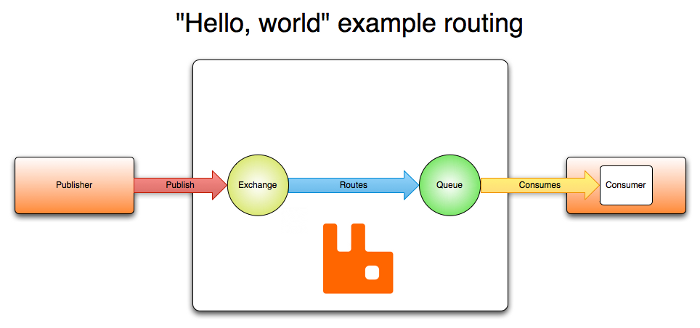
\includegraphics[width=\linewidth]{05-amqp/figuras/fig001}
\caption{Ejemplo de enrutamiento en AMQP}
\label{fig:figura1}
\end{figure}

Cuando se publica un mensaje, se pueden especificar diferentes atributos (\emph{metadata}).
Alguno de estos atributos pueden ser usados por el \emph{broker}, sin embargo,
el cuerpo del mensajes es completamente opaco para el \emph{broker} y sólamente
será usado por la aplicación que recibirá el mensaje.

Las redes pueden tener problemas y las aplicaciones puede fallas al procesar los
mensajes, por eso mismo, el modelo \texttt{AMQP} hace uso de \texttt{ACKs}. Cuando
un mensaje se entrega a un consumidor, éste debe notificar al broker que ha procesado
el mensaje, ya sea de forma automática o cuando el desarrollador de la aplicación
lo decida. El \emph{broker} sólamente eliminará el mensaje de la cola cuando
éste haya sido confirmado.

En algunas situaciones, por ejemplo, cuando un mensaje no puede ser enrutado,
el mensaje puede ser devuelto al productor, descartado o, si el broker lo implementa,
enviado a una cola especial llamada \emph{dead letter queue}. Los consumidores pueden
elegir cómo manejar situaciones como estas usando algunos parámetros a la hora de
publicar los mensajes.

Las colas, los \emph{exchanges} y los \emph{bindings} son conocidas como
\textbf{entidades de AMQP}-

\section{\emph{Exchanges}}

Los \emph{exchanges} son entidades de AMQP a donde llegan los mensajes. Éstos
al recibir los mensajes los enrutan hacia cero o más colas. El algoritmo de
enrutado depende del tipo de \emph{exchange} y las reglas definidas (\emph{bindings}).
Existen cuatro tipos de \emph{exchanges}:

\begin{itemize}\itemsep1pt \parskip0pt \parsep0pt
\item Direct exchange: \texttt{amq.direct}
\item Fanout exchange: \texttt{amq.fanout}
\item Topic exchange:	\texttt{amq.topic}
\item Headers exchange:	\texttt{amq.match}
\end{itemize}

Independientemente del tipo de \emph{exchange}, éstos son declarados con ciertos
atributos, los más importantes son:

\begin{itemize}\itemsep1pt \parskip0pt \parsep0pt
\item Name: Nombre del \emph{exchange}.
\item Durability: Indica al \emph{broker} que debe sobrevivir a
reinicios.
\item Auto-delete: Son eliminados sin no hay ninguna cola asociada.
\item Arguments: Dependen del \emph{broker}.
\end{itemize}

\subsection{\emph{Direct Exchange}}

Los \emph{exchanges} directos entregan los mensajes a las colas basándose en
la \texttt{routing key}. Son ideales para enrutamiento \emph{unicast}, aunque
también se pueden usar para \emph{multicast}. Funcionan de la siguiente manera:

\begin{itemize}\itemsep1pt \parskip0pt \parsep0pt
\item Una cola se conecta (establece un \emph{binding}) al \emph{exchange} con
la \texttt{routing key} \texttt{K = R}
\item El \emph{exchange} directo suele ser usado para distribuir mensajes entre
múltiples \emph{workers} en modo \emph{round robin}. Es importante ser conciente
de que en \texttt{AMQP} se balancea entre consumidores y no entre colas.
\end{itemize}

Se puede ver de forma grágica en la \FIG{figura2}.

\begin{figure}[htbp]
\centering
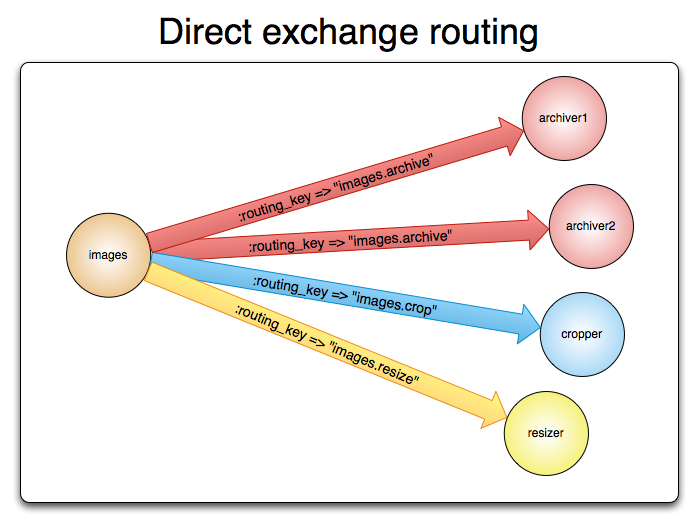
\includegraphics[width=0.75\linewidth]{05-amqp/figuras/fig002}
\caption{\emph{Exchange} directo}
\label{fig:figura2}
\end{figure}

\subsection{\emph{Fanout Exchange}}

Este tipo de \emph{exchange} enruta todos los mensajes a todas las colas con las
que está conectado, es decir, la \texttt{routing key} se ignora en este caso.
Una copia de cada mensaje es enviado a cada una de las colas. Este tipo de
\emph{exchange} es ideal para el tráfico \emph{broadcast}.

Se puede ver de forma grágica en la \FIG{figura3}.

\begin{figure}[htbp]
\centering
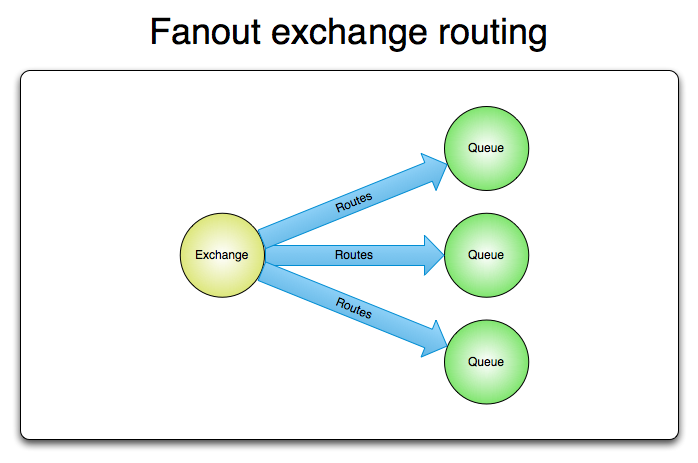
\includegraphics[width=0.75\linewidth]{05-amqp/figuras/fig003}
\caption{\emph{Fanout exchange}}
\label{fig:figura3}
\end{figure}

\subsection{\emph{Topic Exchange}}

En este caso, los mensajes se envían a una o varias colas, basándose en la
\texttt{routing key} con la que una cola está conectada a un \emph{exchange}. Este
patrón se suele usar en modelos de publicador/suscriptor.

\subsection{\emph{Header Exchange}}

El \emph{header echange} está diseñado para enrutar mensajes basándose en múltiples
atributos que viajan en las cabeceras de los mensajes en lugar de usar la
\texttt{routing key}.

\section{Colas}

Las colas en \texttt{AMQP} son muy similares a las colas en otros sistemas de
colas. Almacenan mensajes que pueden se consumidos por aplicaciones. Las colas
comparten algunas propiedades con los \emph{exchanges}, pero también tienen sus
propios atributos:

\begin{itemize}\itemsep1pt \parskip0pt \parsep0pt
\item Name: Nombre de la cola.
\item Durable: Indica al \emph{broker} que deben sobrevivir a
reinicios.
\item Exclusive: Sólo se permite una conexión a la cola.
\item Arguments: Dependen del \emph{broker}.
\end{itemize}

Las colas deben ser declaradas antes de poder ser usadas. La declaración hace que
la cola se cree si no existía anteriormente, si ya estuviese declarada, otra
declaración no tendrá ningún efecto. Si se vuelve a declarar con otros atributos
diferentes, se producirá una excepción.

\subsection{Colas durables}

Las colas durables se persisten a disco y sobreviven a reinicios del \emph{broker},
en cambio, las colas que no son durables son llamadas transitorias. No todos los
escenarios requieren que una cola sea durable.

La durabilidad de una cola no hace que los mensajes que sean enrutados hacia esa
cola sean durables. Si el \emph{broker} se reinicia, las colas durables volverán
a declararse durante el inicio de forma automática, sin embargo, sólamente los
mensajes persistidos podrán recuperarse.

\section{\emph{Bindings}}

Los \emph{bindings} son reglas usadas por los \emph{exchanges} para enrutar los
mensajes recibidos hacia las colas. Para que un \emph{exchange} enrute un mensaje
a una cola, dicha cola debe enlazarse con el \emph{exchange}. Los \emph{bindings}
pueden tener atributos opcionales como las \texttt{routing keys}. La finalidad
de una clave de enrutado es seleccionar ciertos mensajes publicados en un \emph{exchage}
que está enlazado con una cola, es decir, actúan como filtros.

Cuando un mensaje no se puede enrutar hacia una cola se descartará o se devolverá
al productor, dependiendo de los atributos que el productor haya ajustado.

\section{Mensages}

Los mensajes en \texttt{AMQP} tienen atributos. Algunos de ellos son tan común
que la especificación los define de forma que los desarrolladores no tienen que
preocuparse por ellos.

\begin{itemize}\itemsep1pt \parskip0pt \parsep0pt
\item Content type
\item Content encoding
\item Routing key
\item Delivery mode
\item Message priority
\item Message publishing timestamp
\item Expiration period
\item Publisher application id
\end{itemize}

Algunos atributos los usa el \emph{broker}, pero la mayoría de ellos son para
los consumidores que lo reciben. Algunos atributos
son opcionales. Los atributos se fijan cuando el mensaje se publica.

Los mensajes también tienen una carga (los datos) que el \emph{broker} trata
como una ristra de \emph{bytes}. El \emph{broker} no inspecciona o modifica
los datos. Es bastante común enviar los datos serializados en formatos como
\texttt{JSON}, \texttt{MessagePack}, \texttt{Protocol BUffers}, etc. Para comunicar
esta información se pueden usar los atributos \texttt{content-type} o \texttt{content-encoding}.

Los mensajes pueden ser publicados como persistentes, que hace que el \emph{broker}
los persista a disco. Si el servidor se reinicia, el sistema se asegura que los
mensajes persistentes no se pierdan. Sólo por publicar un mensaje en un \emph{exchange}
durable o que la cola a la que el mensaje es enrutado sea durable no hace que el
mensaje sea persitido, para ello el mensaje tiene que ser publicado como persistente.
Hay que tener en cuenta que publicar mensajes persistentes afecta al rendimiento.
